\chapter{Propuesta para CMMN}
\label{aplica}

Se retoma aquí el grafo que se genera al modelar un Caso con la notación CMMN. De tal esquema surge esta propuesta. La figura \ref{CMMN_modelo} presentada antes será la base para este ejemplo. 

\begin{figure}[h]
  \centering
    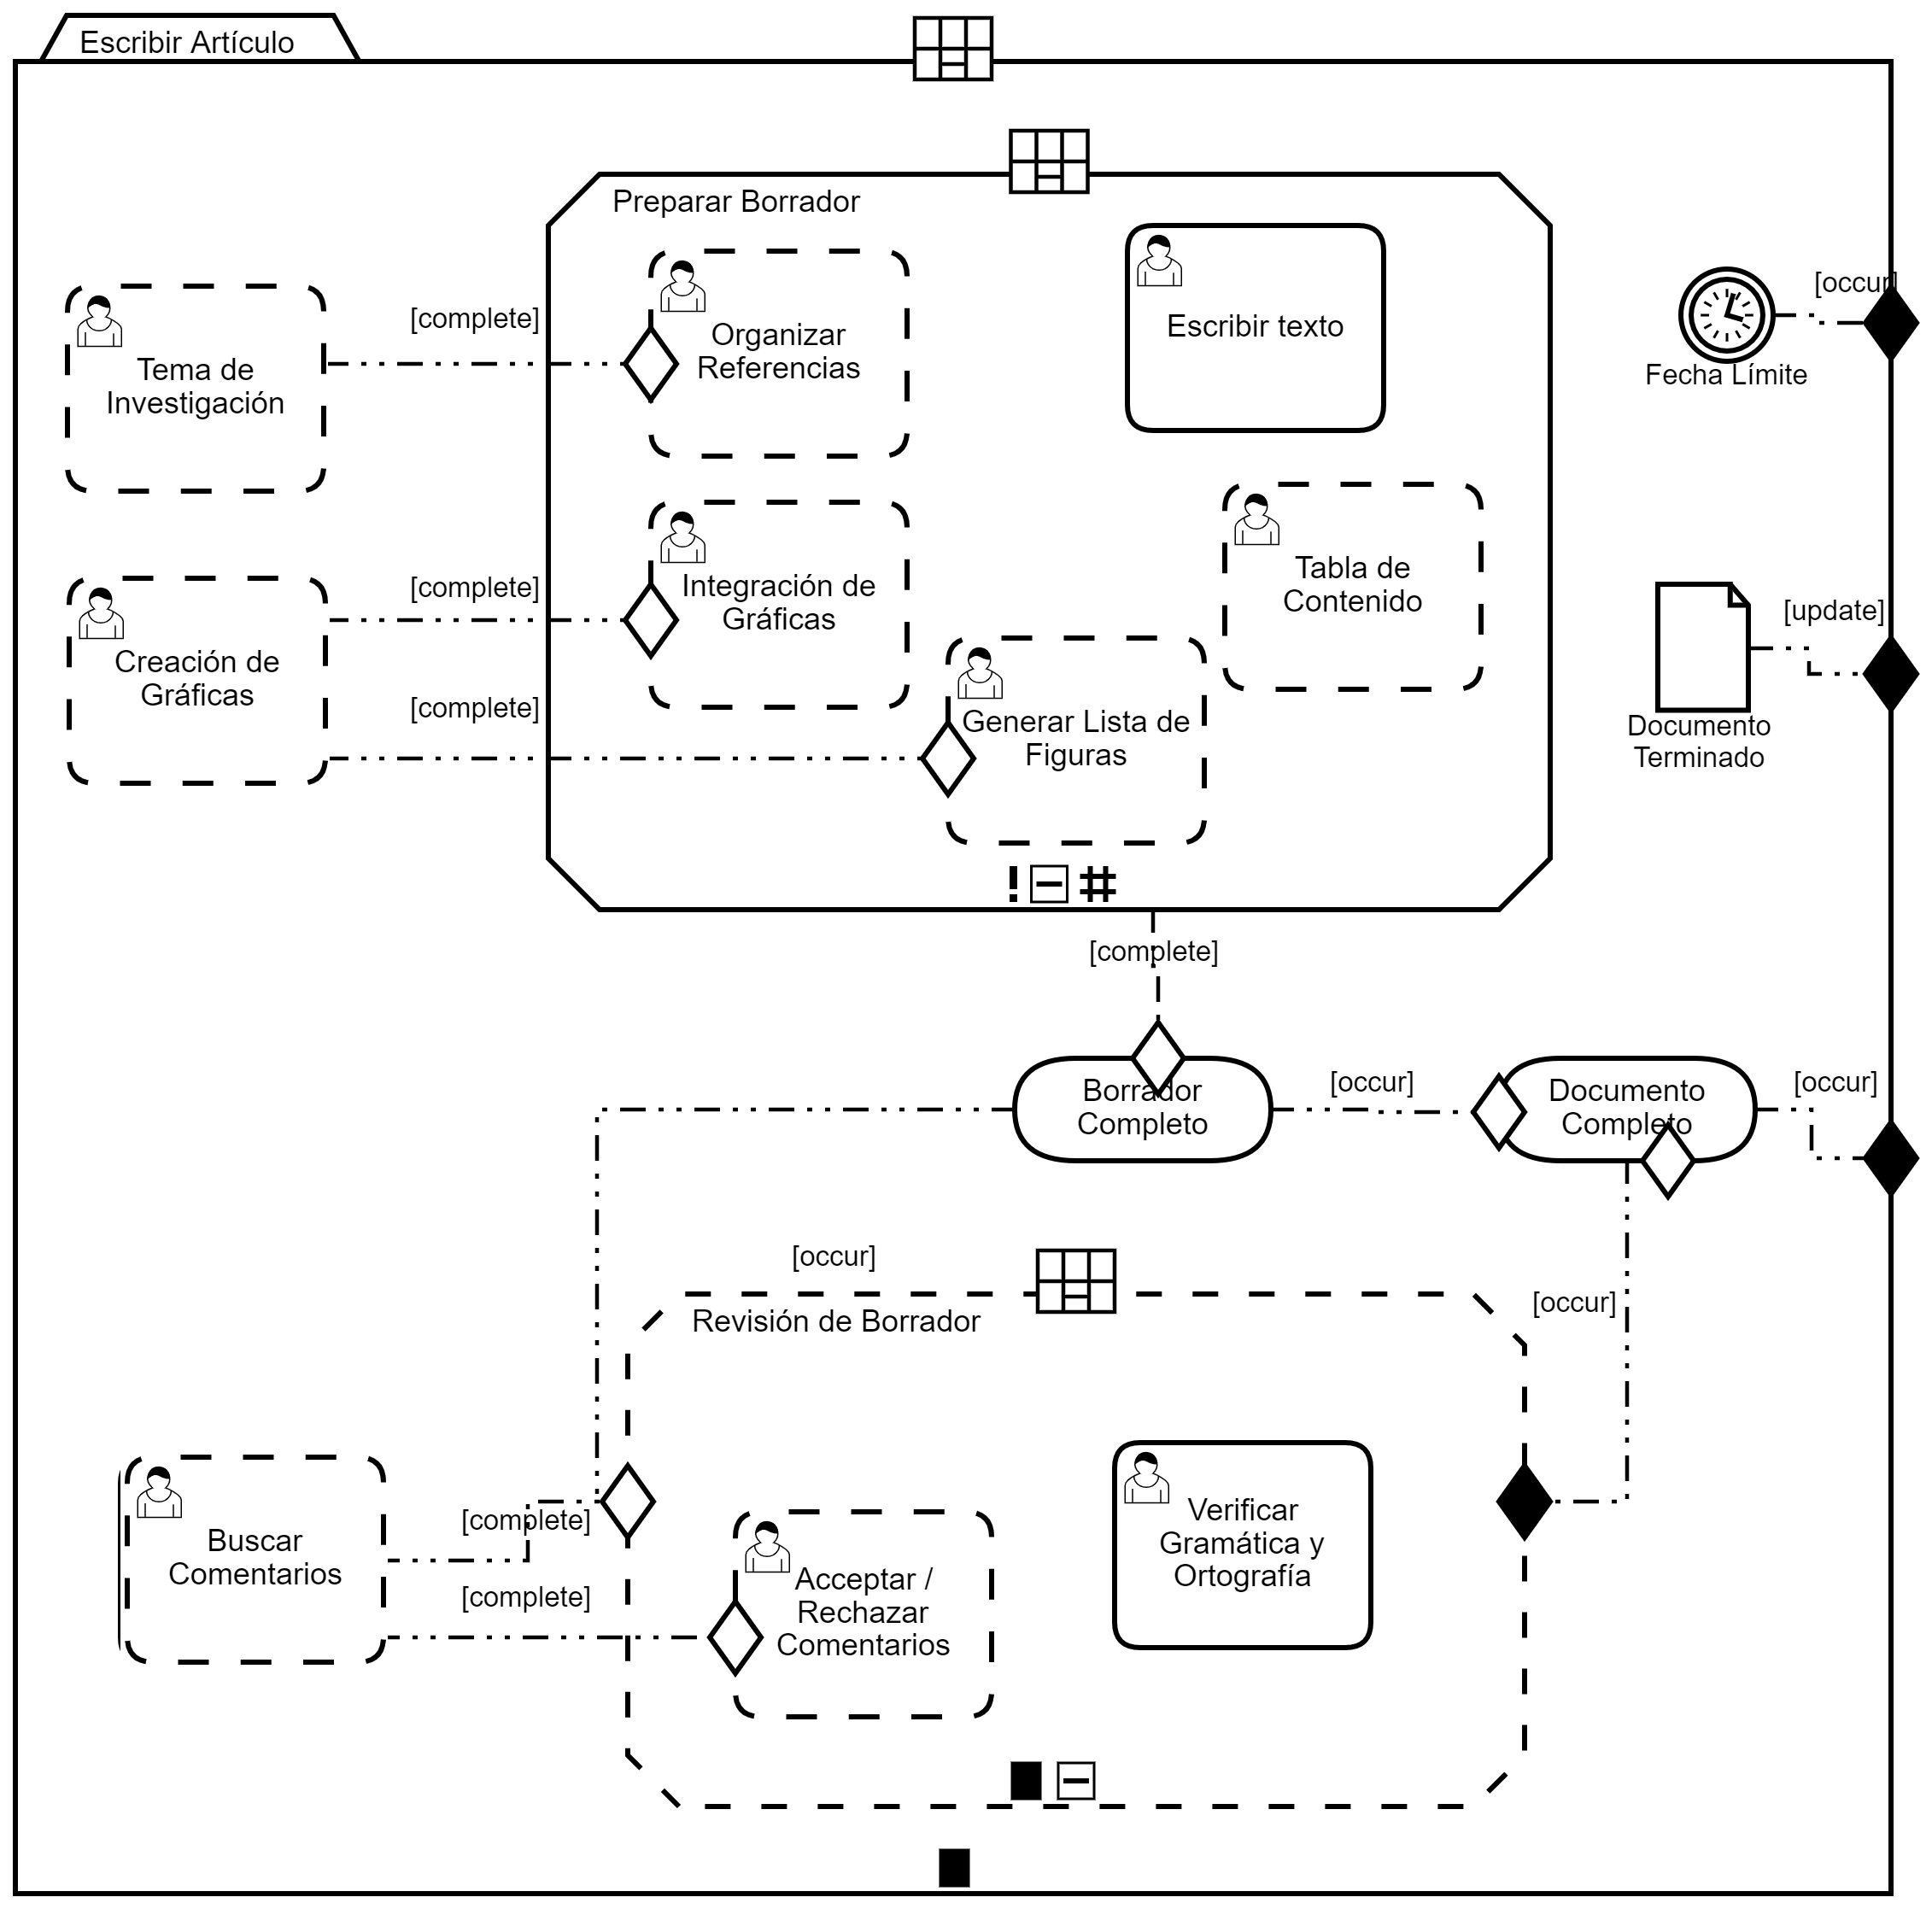
\includegraphics[scale=0.25]{ModeloCMM.png}
  \caption[Modelo CMMN]{Grafo en CMMMN que se llevará al modelo propuesto}
  \label{CMMN_modelo}
\end{figure}


\section{Modelo CMMN en un grafo por etapas}

Es importante recordar que las líneas punteadas de la figura \ref{CMMN_modelo} representan que la secuencia que se puede seguir o la presencia de algunas actividades es posible, pero no determinista.

Se vislumbra entonces, cómo esta notación CMMN puede llevarse al grafo con etapas propuesto, donde se pueda modelar la incertidumbre presente en la selección de tareas, disponiendo en cada etapa el conjunto de actividades posibles, para que el algoritmo de aprendizaje recomiende la tarea a seguir de la siguiente etapa.

Para esto se propone:

\begin{itemize}
    \item Si dostareas b y c están después de una tarea a, pero b y c no son disjuntas, entonces se deben ofrecer b y c en cualquiera de las etapas siguientes.
    \item Colocar una actividad nula en cada etapa para cuando no se ha de tomar alguna.
    \item Dejar las aristas suficientes para las posibles conexiones entre nodos, sin ocuparse demasiado por los prerrequisito, puesto que el algoritmo ha de aprender cuando los caminos no sean viables.
\end{itemize}


La figura \ref{CMMN_modelo} representa las tareas para escribir un artículo. En ella se pueden diferenciar claramente dos partes concernientes a la preparación del borrado y a su revisión. Estas partes permiten separar en dos figuras el grafo resultante de la propuesta de esta tesis.

Los grafos que se generaron a partir de esas apreciaciones se presentan en las figuras \ref{CMMN_modelo1} y \ref{CMMN_modelo2}.

\begin{figure}[h]
  \centering
    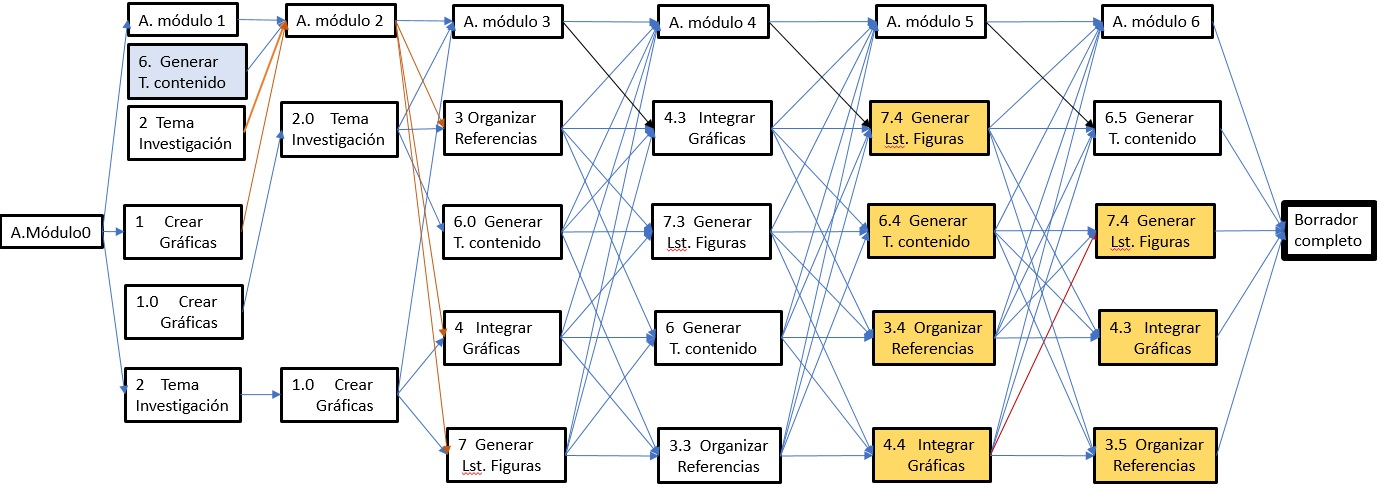
\includegraphics[scale=0.5]{DeCMMN1.jpg}
  \caption{Caso en etapas. Parte 1.}
  \label{CMMN_modelo1}
\end{figure}


\begin{figure}[h]
  \centering
    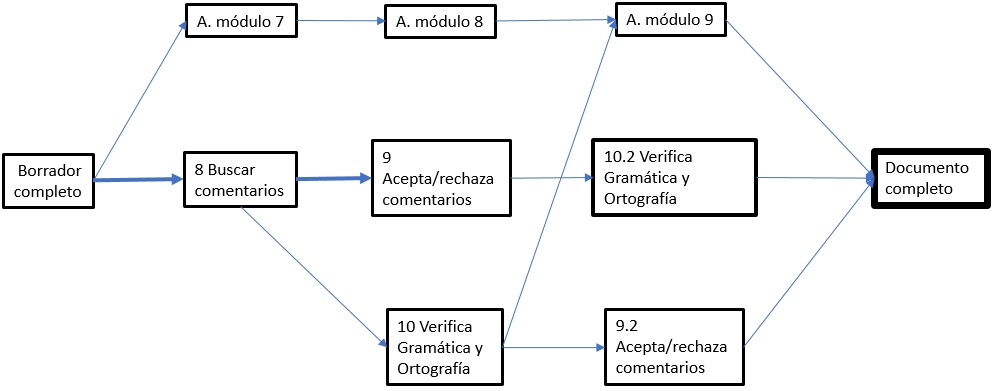
\includegraphics[scale=0.55]{DeCMMN2.jpg}
  \caption{Caso en etapas. Parte 2.}
  \label{CMMN_modelo2}
\end{figure}


También se ha considerado, para cuando se hace necesario traer de alguna forma la información pasada de actividades pasadas, que son predecesoras de otras, mediante la activación de una bandera que lo indique. Así mismo se analizó la posibilidad de fusionar actividades no disyuntas en un nodo ficticio, con la salvedad de que no es fácil esclarecer con certeza sus prerrequisitos.
%Un caso específico se presenta en el apéndice \ref{apendicecaso}, el cual se constituye como una parte del trabajo de investigación en el manejo de casos dinámicos de las BPMS que concibió el ingeniero Luis Chaparro, al interior del grupo de investigación GIPROCAS de la Universidad de Boyacá en Colombia.

%Dada esta introducción al caso de estudio, se procede a presentar las consultas bibliográficas correspondientes para establecer si el grafo propuesto ya se encuentra en otra investigación y si ya ha sido abordado un modelo cercano al \textit{L-n-armed-bandits}.